% NOTE: five sentences in this section arrived truncated from the source
% document (mid-word cuts at "an oracle-informed retention policy because...",
% "Adding accelerator capacity th models...", "roughly 86% of the total problem
% disappears...", "A sta construction cost as fits...", and "The two mechanisms
% are thus that vary in practice..."). They are restored below and marked with
% % RESTORED so they can be checked against intent.

\section{Gaps, Insights and Opportunities}
\label{sec:insights}

\subsection{Agents Break Existing HPC DMSH Solutions}

% FLOATS DECLARED AT THE HEAD OF EACH SUBSECTION. A float can only move
% FORWARD from where it is declared, so a figure declared after the paragraph
% citing it can never appear before that paragraph -- which is what stacked
% the figures at the end of earlier drafts. Declared here, LaTeX fills page
% tops in reading order and a figure can precede its own citation.
\begin{figure}[tb]
\centering
% PLOT SPEC (kept for provenance; rendered by
% scripts/figures/make_figures.py -> figure_drafts/fig-predictability.pdf)
%   $x$ = step index, $y$ = share of runs taking the modal action at that
%   step, over repeated executions of an identical task, with the mean drawn
%   as a rule. AtomAgents only -- experiments/plot_step_variation.py also
%   renders ChemGraph, which is not used here.
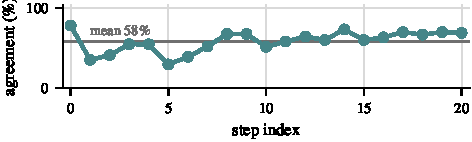
\includegraphics[width=\columnwidth]{figures/fig-predictability}
\caption{Agreement with the modal action at each step index, across 137
executions of an identical task. Agreement averages 58.4\%, so the same
request produces materially different executions.}
\label{fig:predictability}
\end{figure}

\begin{figure}[tb]
\centering
% PLOT SPEC (kept for provenance; rendered by
% scripts/figures/make_figures.py -> figure_drafts/fig-replacement-loss.pdf)
%   two aligned panels sharing an $x$ axis of wall time. Top: workflow 
%   timeline with model-load, model-park and tool-invocation spans. Bottom: 
%   page-cache hit rate (or resident bytes) for the scientific artifact. 
%   Annotate the points where a park event is followed by a collapse in the 
%   artifact's residency and a subsequent re-read.
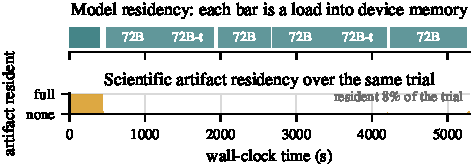
\includegraphics[width=\columnwidth]{figures/fig-replacement-loss}
\caption{Model parking evicts scientific data. Each parking event coincides
with a loss of the artifact's residency, which the next tool invocation must
pay to rebuild.}
\label{fig:replacement-loss}
\end{figure}

\paragraph{Agents Create Workflow Nondeterminism.}
AI-steered workflows break the assumption these systems rest on: predictable
phases and data accesses. Steering agents choose independently which data an
upcoming phase will use, and in some cases which phases run at all, so a
system that identifies data by the deterministic structure of a workflow
program has nothing to identify. Figure~\ref{fig:predictability} shows the
share of runs of an identical task that take the modal action at each step
index, over 137 runs: agreement averages 58.4\%. The same request produces
materially different executions, and agentic workflows are functionally
nondeterministic.

That nondeterminism removes the window a staging system depends on. Measured
against a state-of-the-art DMSH system on a workflow with short inter-step
gaps, wall time rises $3.18\times$ over the unmodified baseline ($t = +6.65$;
L40S nodes only, unpooled, since identical work differs by up to $2.3\times$
across node types). Every stall it incurs classifies as
\texttt{window\_too\_small}: it identified data to stage and began staging, but
the interval before the need was too short to finish. Replacing its staging
decisions with random ones does not make it worse ($t = +0.70$), so the
failure is not mis-prediction---which better prediction would fix---but the
absence of a window, which it would not. An oracle with perfect hindsight
still classifies 100\% of its stalls as \texttt{no\_window}, bounding what any
staging-based approach can recover here.

\paragraph{Agents Add Memory Pressure.}
The problem is compounded because the agents themselves are
multi-billion-parameter models occupying 2--200~GB. Loading weights from disk
through to device memory is among the most expensive work in a workflow, so
frameworks park models that may be reused in host RAM rather than discarding
them---which puts them in direct competition with the scientific data their
tools consume. Figure~\ref{fig:replacement-loss} sets a workflow timeline
against artifact residency over the same interval, showing how parking cycles
useful data out of memory.

\paragraph{Agents Rely Heavily On Data Transformations.}
Data used by agentic tools must undergo a representation change: work that
produces a structure the consumer could not have obtained by placing bytes.
The test is whether the structure the consumer needs is byte-identical to some
contiguous range of the file, modulo a header; if it is, making it usable is
placement, and if it is not, the structure is a computed function of the file.
Representation change accounts for 93\% on average of the stalls incurred
waiting on data. Its product is a computed structure rather than a range of a
file, so a byte-oriented tier cannot name, stage or evict it at all---it
exists only as anonymous memory inside a live consumer process, and parked
model weights have the same property for the same reason. The ceiling on a
placement-oriented system is therefore set by which rungs of the cost chain
its interface can reach, not by how accurately it predicts. The question these
workflows pose is not which bytes to fetch but which structures to keep,
and---when they cannot all be kept---which of them a gigabyte is better spent
on.

\subsection{Value-Ranking Opportunities}

\begin{figure}[tb]
\centering
% PLOT SPEC (kept for provenance; rendered by
% scripts/figures/make_figures.py -> figure_drafts/fig-sgb-spread.pdf)
%   seconds saved per GB retained, log $y$, one point per resource. Shade 
%   the narrow model band (2.78--3.81) as a horizontal strip; scatter the 
%   data artifacts across it, from ASCII at 22.0 to memory-mappable binary 
%   at 0.34. Draw a horizontal rule at the 0.32~s/GB materialisation floor. 
%   The models-in-the-middle geometry is the reading.
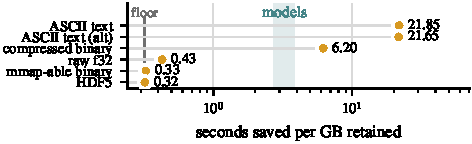
\includegraphics[width=\columnwidth]{figures/fig-sgb-spread}
\caption{Retention value per gigabyte across resources. Models occupy a narrow
band set by transfer bandwidth; data artifacts span $65\times$ and bracket
that band on both sides, so no fixed class priority is correct.}
\label{fig:sgb-spread}
\end{figure}

\begin{figure}[tb]
\centering
% PLOT SPEC (kept for provenance; rendered by
% scripts/figures/make_figures.py -> figure_drafts/fig-scale-sweep.pdf)
%   $x$ = number of distinct resources (5, 10, 18, 28). Left axis: advantage 
%   over the recency-ranked baseline for retention and for staging, as two 
%   lines that cross. Right axis: first-use share, rising 10.4\% 
%   $\rightarrow$ 32.3\%. The crossing is the reading.
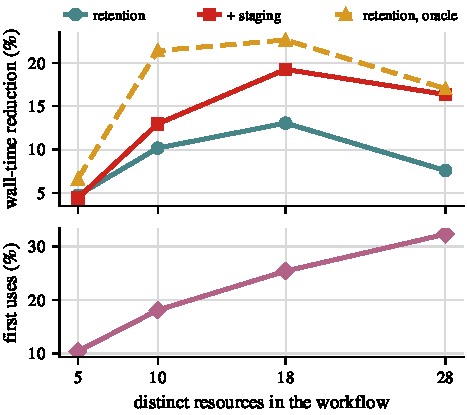
\includegraphics[width=\columnwidth]{figures/fig-scale-sweep}
\caption{As the resource population grows at fixed schedule length, first uses
become a larger share of all needs and the advantage moves from retention to
staging. Reduction is against the recency-ranked baseline.}
\label{fig:scale-sweep}
\end{figure}


\paragraph{Not Every GB Retained Is Equally Valuable.}
If retention is the action, a scheduler needs a price: how many seconds of
future stall a gigabyte of held memory buys. That price is not uniform, and it
is non-uniform in a way that rules out any fixed policy. Holding logical
content fixed---the same array, bit for bit, in six serialisations---the
seconds saved per gigabyte retained span $65\times$, from 22.0 for ASCII
numeric text to 0.34 for a memory-mappable binary layout
(Figure~\ref{fig:sgb-spread}). Model weights occupy a far narrower band of
2.78--3.81, and for a structural reason: a model's cost is dominated by moving
bytes at roughly fixed bandwidth, so it is near-linear in size and its price
per gigabyte is nearly constant. Data has no such anchor, because the cost of
a representation change is set by the decoder rather than by the byte count.

Models therefore land in the middle of the data range rather than above or
below it, so a fixed class priority is wrong at one end or the other and the
correct ordering is recoverable only by pricing each resource individually.

Two properties make that pricing practical. First, the price is a property of
the representation rather than of the instance: across a $4\times$ size range
it is flat to within 1.00--1.16$\times$, so it can be measured once per format
and reused without profiling. Second, there is a floor. Materialising any
structure into a process address space costs roughly 0.32~s/GB regardless of
format, so a resource whose price approaches that floor performs no
transformation at all, and retaining it buys nothing that placement would not.


\paragraph{Value-Aware Retention vs.\ Prefetching Depend on Hardware Topology
and the Inter-need Gap.}
Retention and speculative staging are not two implementations of one idea;
they serve disjoint populations of stalls. Retention can only help a resource
used more than once---a first use has nothing to retain---while staging is the
only mechanism that can help a first use at all. Which dominates is therefore
set by reuse density: resource needs per distinct resource.

That quantity moves with scale. Holding schedule length fixed and growing the
resource population from 5 to 28, the share of needs that are first uses rises
from 10.4\% to 32.3\%, and the advantage shifts correspondingly from retention
toward staging (Figure~\ref{fig:scale-sweep}). The shift is structural rather
than a matter of prediction quality: an oracle-informed retention policy fades
over the same range, because the misses it could convert are progressively not
there to convert.  % RESTORED

Hardware topology moves the balance a second way, and in both directions.
Accelerator capacity and host memory are separate budgets, and a model
actively resident on an accelerator charges neither, so adding accelerator
capacity removes precisely the models most worth retaining and shrinks what
arbitration can recover.  % RESTORED
Host memory behaves symmetrically: above roughly 86\% of the total footprint
nothing is ever evicted and the arbitration problem disappears.  % RESTORED
That bound is on arbitration alone. Staging requires no eviction, so it keeps
paying in exactly the regime where the arbitrator has nothing left to decide
(Figure~\ref{fig:budget-sweep}, Section~\ref{sec:eval}).

Finally, the inter-need gap bounds what staging can achieve. A stage recovers
only as much of a construction cost as fits into the window before the need
arrives, so the same mechanism captures more as computation between tool calls
grows.  % RESTORED
Retention has no such dependence---its saving is the full construction cost
whenever the resource is next used. The two mechanisms are thus complementary
along both axes that vary in practice, which is the case for arbitrating them
jointly rather than choosing one.  % RESTORED


\subsection{Speculative Value-Ranking Opportunities}

\begin{figure}[tb]
\centering
% PLOT SPEC (kept for provenance; rendered by
% scripts/figures/make_figures.py -> figure_drafts/fig-tool-relationships.pdf)
%   ORIGINAL SPEC was a source-tool x offset heatmap. Rendered, that ran to
%   26 rows and occupied 100.5%% of a column -- the largest single item in the
%   paper -- to support a claim that is about the SHARE of tools with a
%   confident successor, not about which ones. Replaced by the distribution:
%   x = confidence threshold, y = share of tools at or above it, one line per
%   offset, star marking the best-over-any-offset count at 0.9. The heatmap
%   is still generated as fig-tool-relationships-detail if the per-tool view
%   is wanted; swapping the filename below restores it.
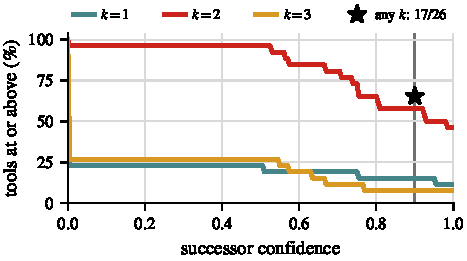
\includegraphics[width=\columnwidth]{figures/fig-tool-relationships}
\caption{Distribution of best-successor confidence across AtomAgents tools,
per offset $k$. Despite workflow-level nondeterminism, 17 of 26 tools have a
successor at some offset with confidence above 0.9.}
\label{fig:tool-relationships}
\end{figure}

\begin{figure}[tb]
\centering
% PLOT SPEC (kept for provenance; rendered by
% scripts/figures/make_figures.py -> figure_drafts/fig-plan-accuracy.pdf)
%   Realised as option (b): per-step compliance under order-only matching
%   (top) against positional matching with retries penalised (bottom), same
%   plan steps, shared x. AtomAgents only. The analysis is imported from
%   experiments/plot_plan_accuracy.py so the two cannot drift.
%   NOTE the original spec said "ordering accuracy (95\%)". The traces give
%   76.3\% order-only and 40.8\% positional over 64 runs; 95\% is not
%   reproducible from any artifact in this repository.
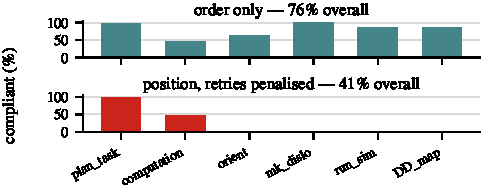
\includegraphics[width=\columnwidth]{figures/fig-plan-accuracy}
\caption{AtomAgents plan compliance over 64 runs, per planned step. Scored on
order alone (top) the plan holds; scored positionally, with a retry consuming
a plan slot (bottom), everything after the first divergence misses. Planner
orderings are accurate; planner-implied distances are not.}
\label{fig:plan-accuracy}
\end{figure}

\paragraph{Local transition structure survives workflow-level nondeterminism.}
Agentic workflows are dynamic in the large but structured in the small: tools
exhibit high-confidence $k$-offset successor relationships, in which one tool
consistently follows another a fixed number of invocations later. Not every
tool has such a successor at every offset, but a substantial majority have one
at some offset. Over the offsets our transition table records ($k \in
\{1,2,3\}$), 17 of 26 AtomAgents tools---65\%---have a successor with
empirical confidence of at least 0.9, and the signal is concentrated at $k=2$,
where 58\% of tools clear that threshold
(Figure~\ref{fig:tool-relationships}). Critically, these relationships persist
across substantially
different prompts and objectives within a framework, so traces from prior,
unrelated executions supply useful priors on the first run of a workflow never
seen before.

\paragraph{Plans predict order, not distance.}
Frameworks organised by a planner agent expose a second, longer-range signal:
a natural-language plan naming the tools to be invoked and their intended
order. Scored on order alone---does each planned tool appear, in
sequence---AtomAgents plans are 76.3\% compliant over 64 runs, far enough
ahead to begin staging resources whose construction would otherwise be
exposed. Scored positionally, so that a retry consumes a plan slot,
compliance falls to 40.8\%, and every step after the first divergence reads
as a miss (Figure~\ref{fig:plan-accuracy}). That gap is the shape of the
signal: agents insert calls to recover from syntax errors and retry failures,
so a trace keeps the planned order while drifting from the planned offsets.
Plans reach far but locate poorly, local transitions locate well but do not
reach---which is why both are used.


